\subsection{Video Classification with Channel-Separated Convolutional Networks}

\subsubsection{Overview}

\begin{itemize}
    \item This paper shows that the amount of channel interactions plays an important role in the accuracy of 3D group convolutional networks.
    \item Factorizes 3D convolutions by separating channel interactions and spatiotemporal interactions as this leads to improved accuracy and lower computational cost.
    \item 3D channel-separated convolutions provide a form of regularization, yielding lower training accuracy but higher test accuracy compared to 3D convolutions.
\end{itemize}

\subsubsection{Background}
\begin{itemize}
    \item \textbf{Group convolution}: In order to reduce the computational cost and model size, the connections can be sparsified by grouping convolutional filters into subsets. Filters in a subset receive signals from only channels within its group.
    \item \textbf{Depthwise convolution}: It is the extreme version of group convolution where the number of groups is equal to the number of input and output channels.     
\end{itemize}

\begin{figure}[H]
    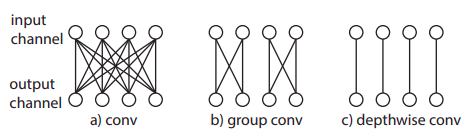
\includegraphics[width=\linewidth]{assets/img/csn_1.png}
\end{figure}

\subsubsection{Architecture}
\begin{itemize}
    \item Channel-separated convolutional networks (CSN) is a 3D CNNs in which all convolutional layers (except for conv1) are either 1×1×1 conventional convolutions or k×k×k depthwise convolutions (where, typically, k = 3).
    \item Conventional convolutional networks model has channel interactions and local interactions (i.e., spatial or spatiotemporal) jointly in their 3D convolutions. The CSN model decomposes these two types of interactions into two distinct layers: 1×1×1 conventional convolutions for channel interaction (but no local interaction) and k×k×k depthwise convolutions for local spatiotemporal interactions (but not channel interaction).
    \item \textbf{Interaction-preserved channel-separated bottleneck block}: It is obtained from the standard bottleneck block by replacing the 3×3×3 convolution with a 1×1×1 traditional convolution and a 3×3×3 depthwise convolution. This block reduces parameters and FLOPs of the traditional 3×3×3 convolution significantly and also  preserves all channel interactions via a newly-added 1×1×1 convolution. 
    \item \textbf{Interaction-reduced channel-separated bottleneck block}: It is derived from the preserved bottleneck block by removing the extra 1×1×1 convolution. This yields the depthwise bottleneck block.. Note that the initial and final 1×1×1 convolutions (usually interpreted respectively as projecting into a lower-dimensional subspace and then projecting back to the original dimensionality) are now the only mechanism left for channel interactions.
\end{itemize}
\begin{figure}[H]
	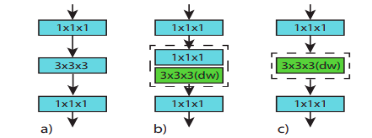
\includegraphics[width=\linewidth]{assets/img/csn_2.png}
	\caption{Standard vs. channel-separated convolutional blocks. (Image courtesy \cite{csn})}
\end{figure}

\subsubsection{Conclusion}
\par CSN-based factorization not only helps to significantly reduce the computational cost, but also improves the accuracy when there are enough channel interactions in the networks